\subsection{Các hệ thống khác của trò chơi}
\subsubsection{Hệ thống cài đặt}
Giao diện cài đặt của trò chơi được hiển thị khi người chơi nhấn vào nút cài đặt, cửa sổ giao diện cài đặt gồm các thông tin như hình dưới:
\begin{figure}[H]
    \centering
    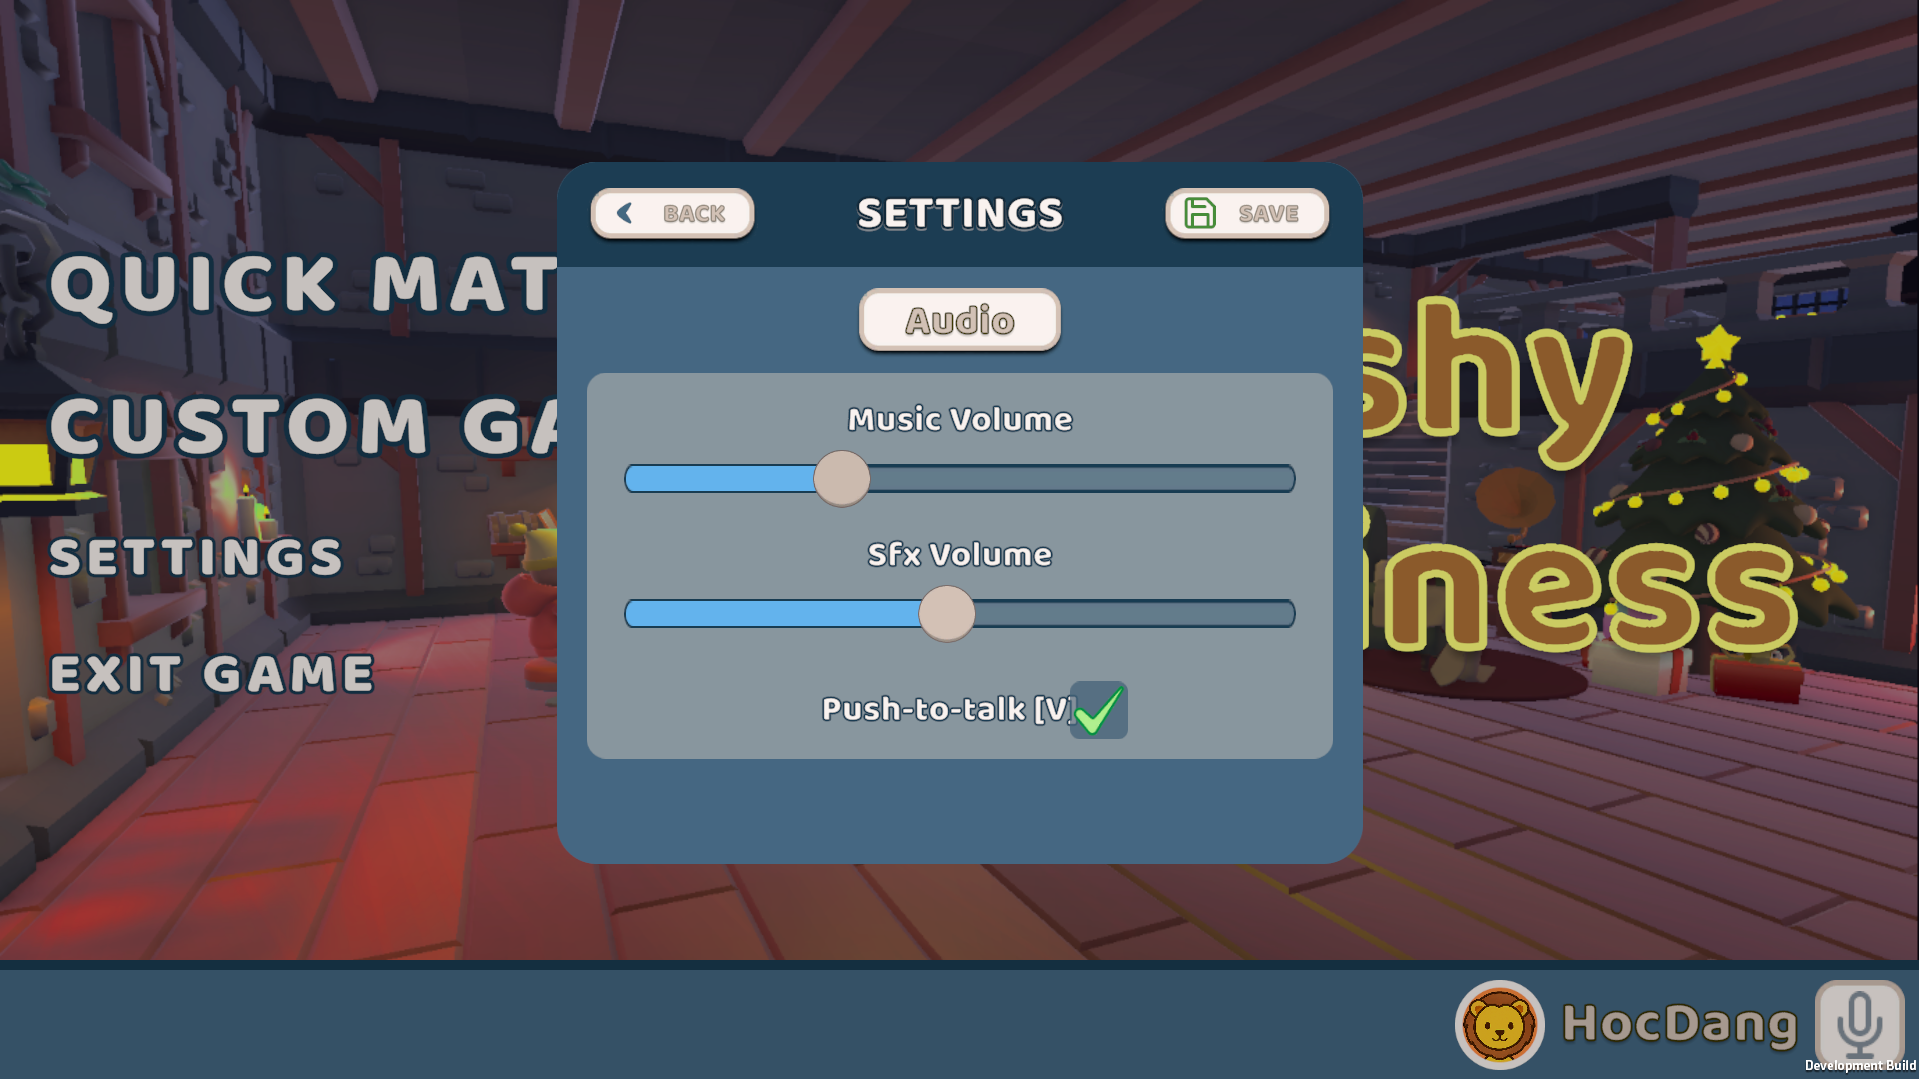
\includegraphics[width=0.75\linewidth]{10.Kết quả/images/Setting.png}
    \caption{Screenshot giao diện cài đặt của trò chơi}
    \label{fig:game-object}
\end{figure}
\begin{itemize}
    \item \textbf{Music Volume}: điều chỉnh âm lượng của nhạc nền
    \item \textbf{Sfx Volume}: điều chỉnh âm lượng của các hiệu ứng âm thanh
    \item \textbf{Push to talk}: tắt/bật chế độ cần phải nhấn giữ nút \textbf{''V''} để nói.
\end{itemize}
\subsubsection{Hệ thống Tooltip}
Khi bạn đang chơi game mà không biết chế độ, vai trò của bạn là gì thì có thể để chuột vào icon, dòng chữ đó để có thể hiện ra \textbf{tooltip}.
\begin{figure}[H]
    \centering
    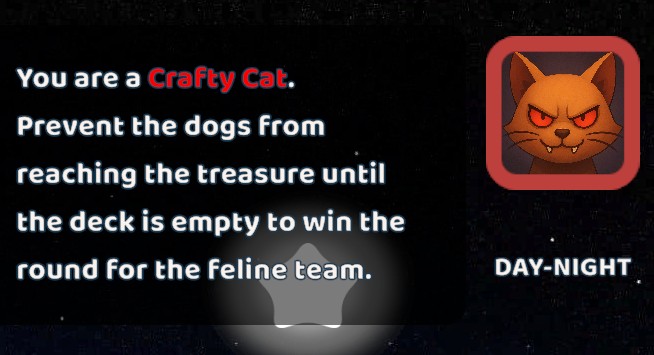
\includegraphics[width=0.75\linewidth]{10.Kết quả/images/CatTooltip.png}
    \caption{Screenshot Tooltip vai trò mèo của trò chơi}
    \label{fig:game-object}
\end{figure}
\begin{figure}[H]
    \centering
    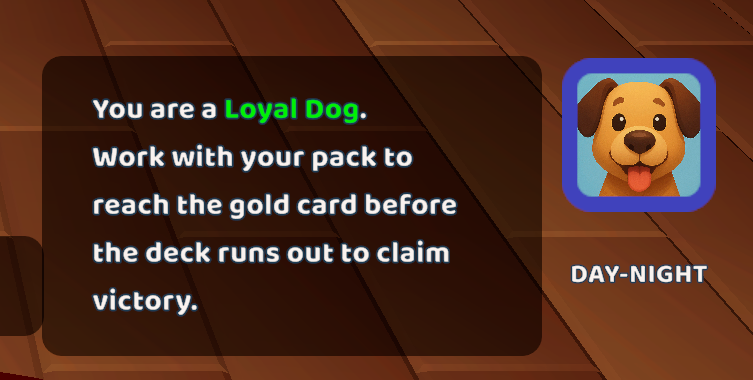
\includegraphics[width=0.75\linewidth]{10.Kết quả/images/DogTooltip.png}
    \caption{Screenshot Tooltip vai trò chó của trò chơi}
    \label{fig:game-object}
\end{figure}
\begin{figure}[H]
    \centering
    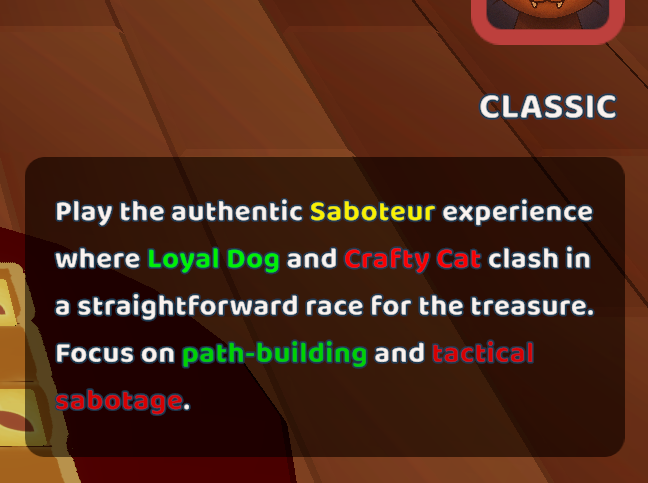
\includegraphics[width=0.75\linewidth]{10.Kết quả/images/ClassicTooltip.png}
    \caption{Screenshot Tooltip chế độ classic của trò chơi}
    \label{fig:game-object}
\end{figure}
\begin{figure}[H]
    \centering
    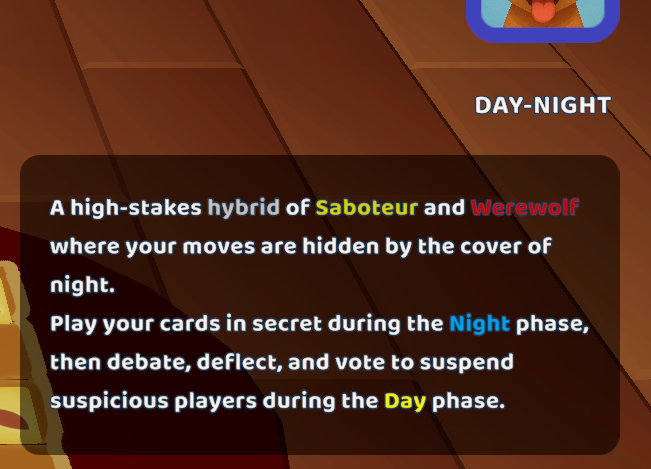
\includegraphics[width=0.75\linewidth]{10.Kết quả/images/DayNightTooltip.png}
    \caption{Screenshot Tooltip chế độ Day Night của trò chơi}
    \label{fig:game-object}
\end{figure}

\subsubsection{Hoạt động ngoài lề}
Người chơi cũng có thể đứng trước gương và nhấn giữ \textbf{''F''} để vào trạng thái thay trang phục, sau khi chọn xong trang phục mình muốn, người chơi có thể nhấn giữ phím \textbf{''F''} để thoát:
\begin{figure}[H]
    \centering
    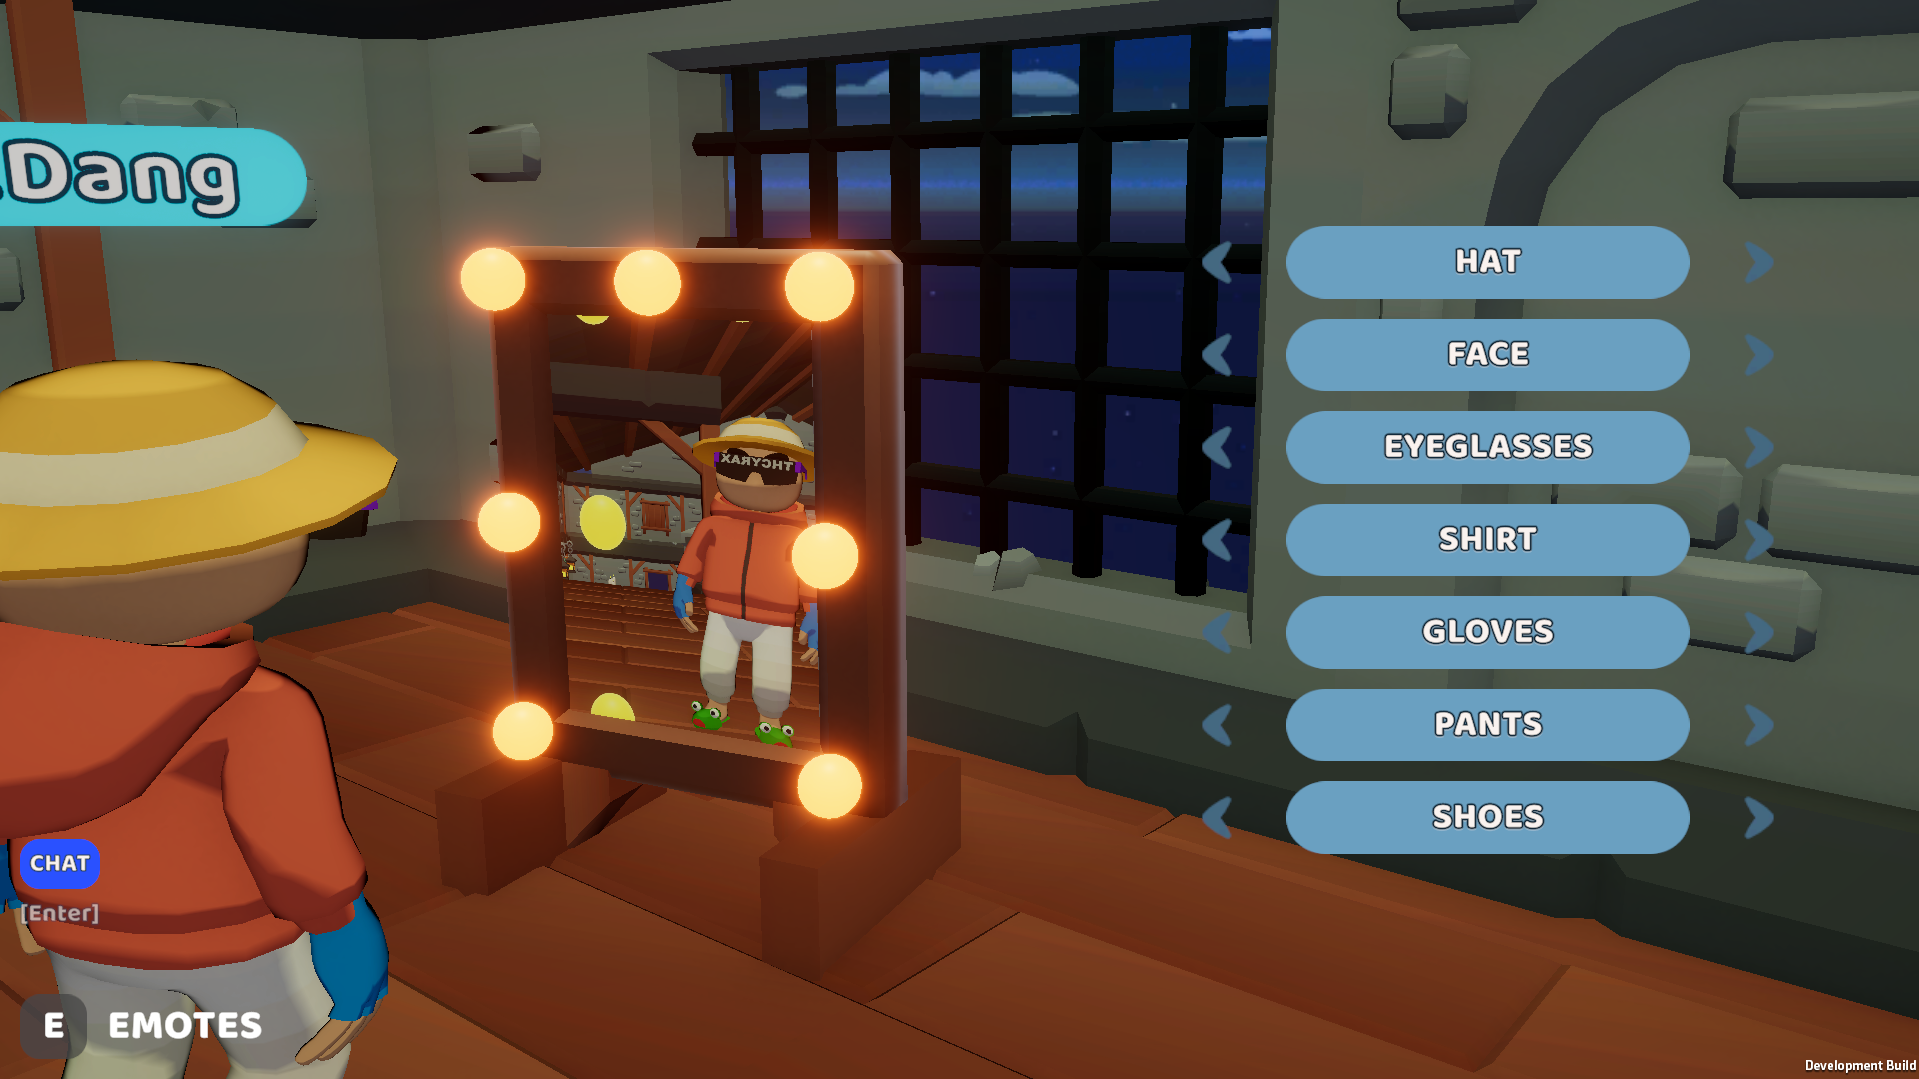
\includegraphics[width=0.75\linewidth]{10.Kết quả/images/ChangeSkin.png}
    \caption{Screenshot màn hình chọn trang phục của trò chơi}
    \label{fig:game-object}
\end{figure}
Hoặc người chơi cũng có thể đến chiếc ghế trước piano và nhấn giữ phím \textbf{''F''} để có thể ngồi vào. Tại đây người chơi có thể bắt đầu tương tác với piano bằng cách nhấn 7 phím đầu tiên của 3 hàng chữ trên bàn phím.
\begin{figure}[H]
    \centering
    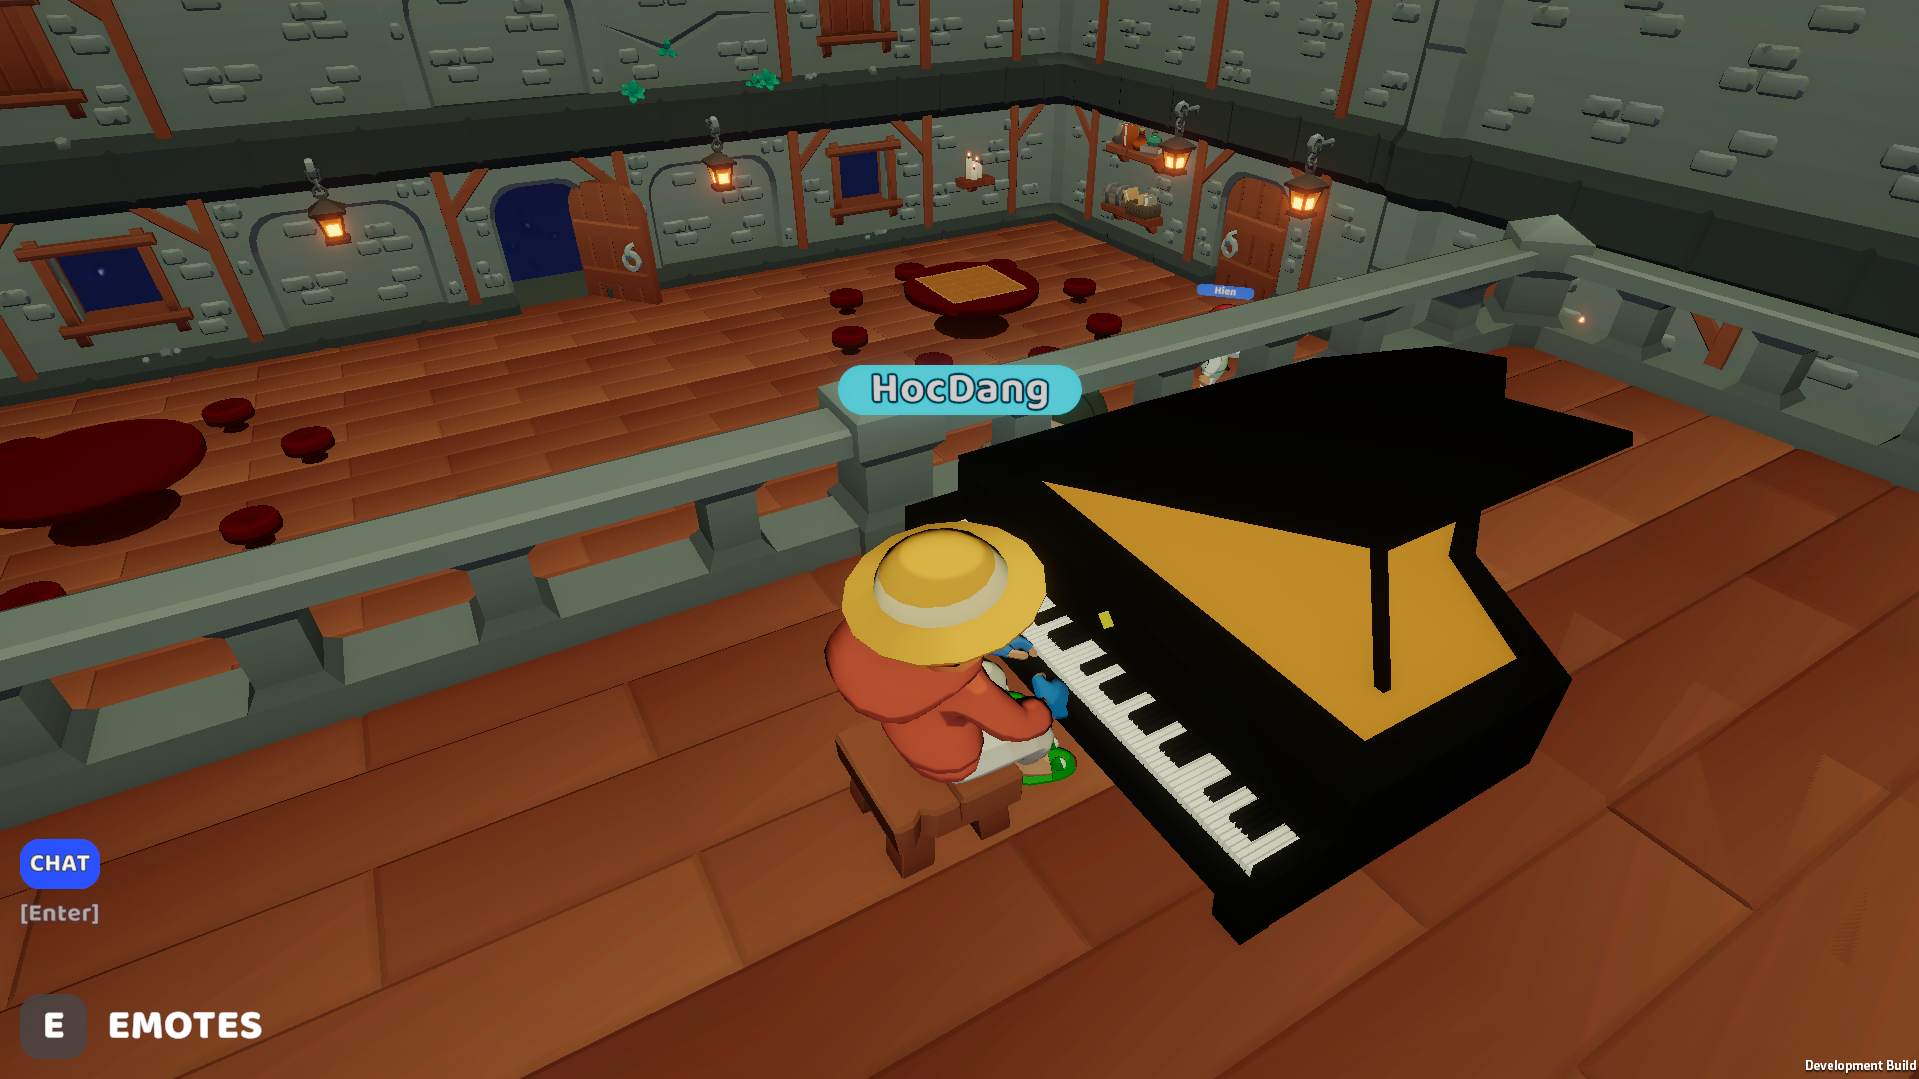
\includegraphics[width=0.75\linewidth]{10.Kết quả/images/PlayPiano.png}
    \caption{Screenshot màn hình chơi piano của trò chơi}
    \label{fig:game-object}
\end{figure}

Hơn nữa người chơi cũng có thể nhấn giữ phím \textbf{''E''} và sử dụng \textbf{lăn chuột} để chọn 1 emote để nhấn vật của người chơi có thể thực hiện một hành động như là nhảy, vẫy tay, ...
\begin{figure}[H]
    \centering
    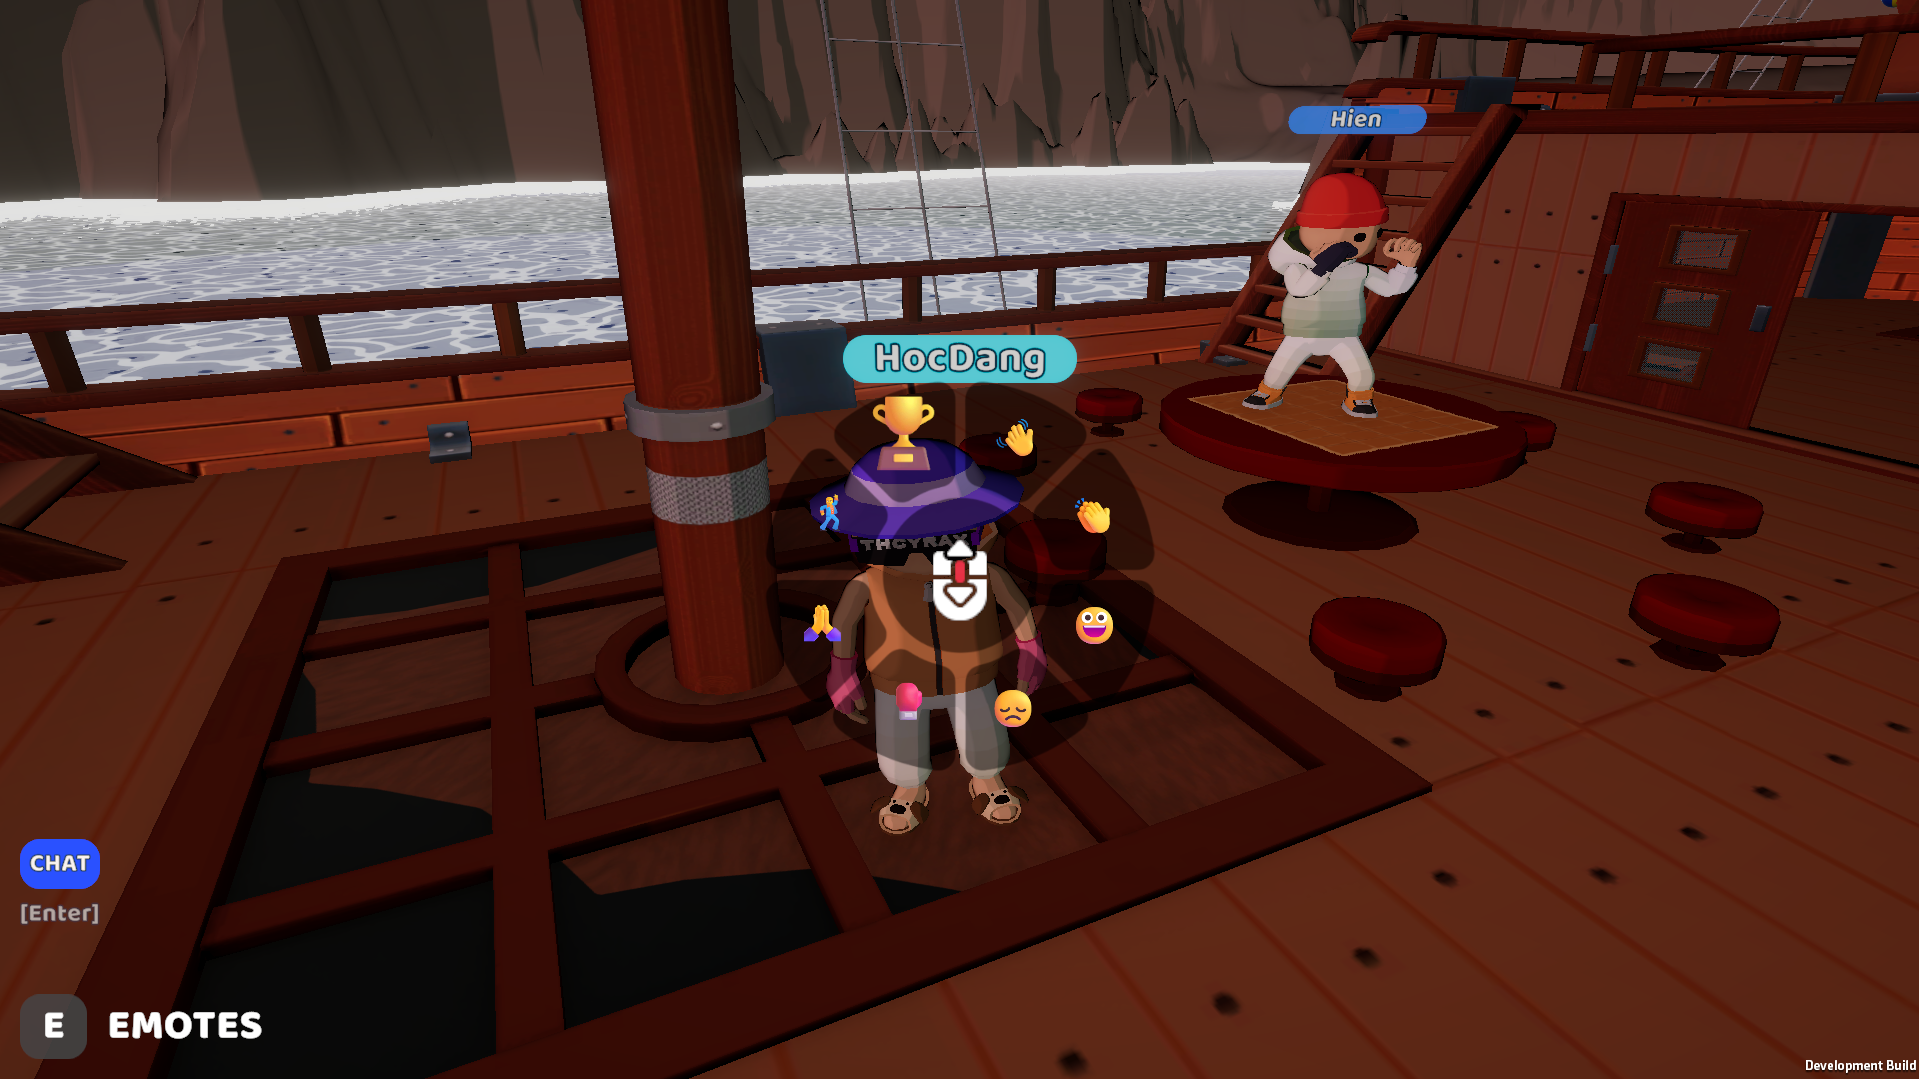
\includegraphics[width=0.75\linewidth]{10.Kết quả/images/Emote.png}
    \caption{Screenshot màn hình Emotes của trò chơi}
    \label{fig:game-object}
\end{figure}

Người chơi cũng có thể nhấn phím \textbf{''Enter''} để mở hộp thoại text chat và bắt đầu chat với những người chơi khác:
\begin{figure} [H]
    \centering
    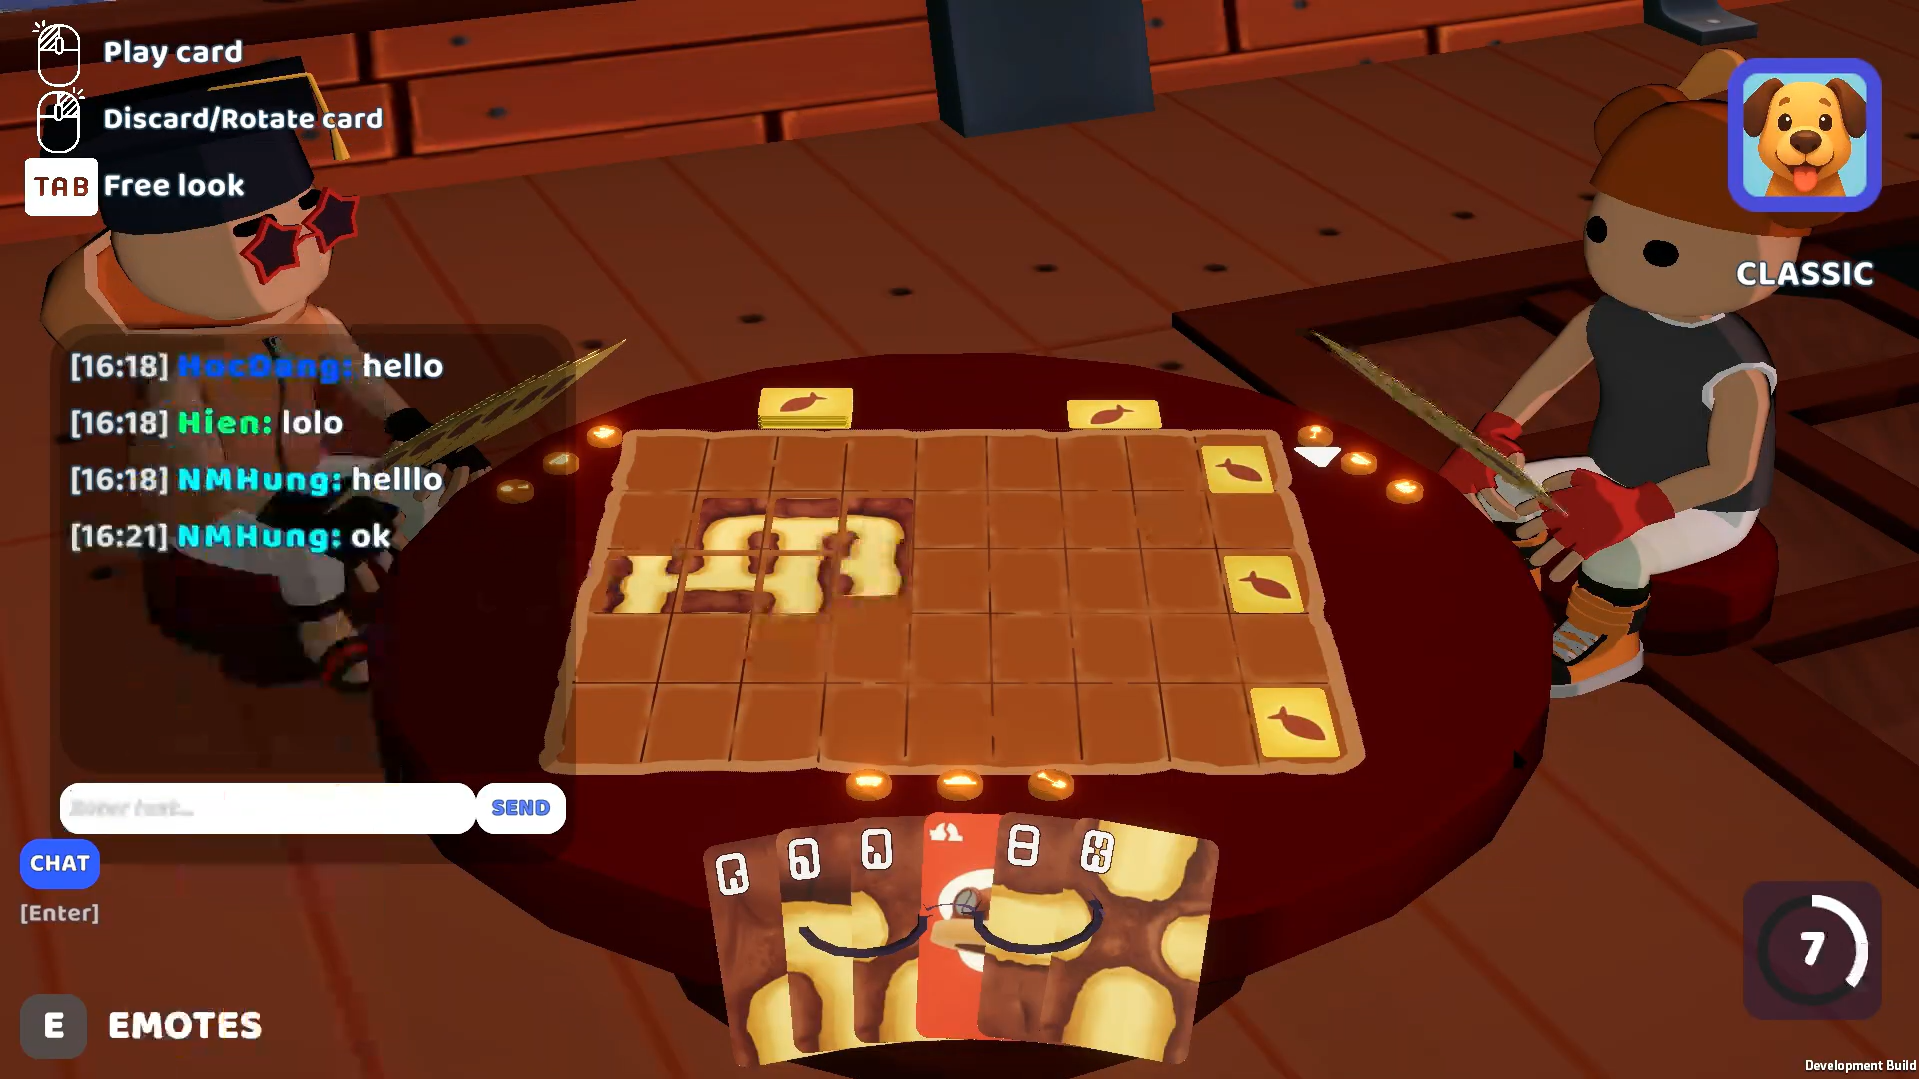
\includegraphics[width=0.75\linewidth]{10.Kết quả/images/TextChat.png}
    \caption{Screenshot màn hình text chat của trò chơi}
    \label{fig:placeholder}
\end{figure}
